\documentclass[10pt]{beamer}
\usetheme{mtec}
\setbeamercovered{transparent}

\usepackage[utf8]{inputenc}

%%%%%%%%%%
% FONTS %
%%%%%%%%%%

%% Default font: lmodern, doesn't require fontspec % solves some default warnings
%\usepackage[T1]{fontenc}
\usepackage{lmodern}            
%\usepackage{sfmath}        % Sans Serif Math, off by default

%% Protects fonts from Beamer screwing with them
%% http://tex.stackexchange.com/questions/10488/force-computer-modern-in-math-mode
\usefonttheme{professionalfonts}


%% XeLaTeX fonts: (comment out if you don't use XeLaTeX)

%% For advanced fonts: access local OS X fonts
%\usepackage[no-math]{fontspec}
%% This template uses typical OS X and Adobe fonts
%\defaultfontfeatures{Mapping=tex-text}  % This seems to be important for mapping glyphs properly

%\setmainfont{Gill Sans MT Pro Book}         % Beamer ignores "main font" in favor of sans font
%\setsansfont{Gill Sans MT Pro Book}         % This is the font that beamer will use by default
% \setmainfont{Gill Sans Light}     % Prettier, but harder to read

%\setbeamerfont{title}{family=\fontspec{Gill Sans MT Pro Book}}


%\newcommand{\handwriting}{\fontspec{augie}} % From Emerald City, free font
% \newcommand{\handwriting}{}   % If you prefer no special handwriting font or don't have augie

%% Gill Sans doesn't look very nice when boldfaced
%% This is a hack to use Helvetica instead
%% Usage: \textbf{\forbold some stuff}
%\newcommand{\forbold}{\fontspec{Helvetica}}
% \newcommand{\forbold}{} % if you want no special boldface


\usepackage{textcomp}
\usepackage{gensymb}
%%%%%%%%%%%%%%%%%%%%%%%%
% Usual LaTeX Packages %
%%%%%%%%%%%%%%%%%%%%%%%%
\usepackage{amsmath}
\usepackage{amssymb}
\usepackage{mathtools}
\usepackage{tabularx}
\usepackage{xcolor}
\usepackage{multirow}
\usepackage{bm}
\usepackage[separate-uncertainty=true]{siunitx}
\sisetup{detect-weight}

\usepackage[ngerman, english]{babel}
\usepackage{graphicx}
\usepackage{epstopdf}
\usepackage{epsfig}
\graphicspath{{../figures/}}
\usepackage{caption}
\usepackage{subcaption}
\captionsetup{compatibility=false}

\usepackage{tikz}
\usepackage{pgfplots}
\usetikzlibrary{shapes,arrows,3d,calc,fit,shadows}
\usepackage{tikz-3dplot}

%\usepackage{animate}
%\usepackage{media9}



\usepackage{hyperref}

\usepackage{xargs}

\makeatletter
\tikzoption{canvas is xy plane at z}[]{%
  \def\tikz@plane@origin{\pgfpointxyz{0}{0}{#1}}%
  \def\tikz@plane@x{\pgfpointxyz{1}{0}{#1}}%
  \def\tikz@plane@y{\pgfpointxyz{0}{1}{#1}}%
  \tikz@canvas@is@plane
}
\makeatother
\tikzset{xyp/.style={canvas is xy plane at z=#1}}
\tikzset{xzp/.style={canvas is xz plane at y=#1}}
\tikzset{yzp/.style={canvas is yz plane at x=#1}}

%%% Axes orientation for the Scanner Arrangement
\newcommandx*{\axisorientation}[7][1=220,2=-20,3=90,4=0.75,5=1,6=no]{
  \renewcommand{\xangle}{#1}
  \renewcommand{\yangle}{#2}
  \renewcommand{\zangle}{#3}

  \renewcommand{\xlength}{#4}
  \renewcommand{\ylength}{#5}
  \renewcommand{\zlength}{#7}
  \renewcommand{\lab}{#6}

  \pgfmathsetmacro{\xx}{\xlength*cos(\xangle)}
  \pgfmathsetmacro{\xy}{\xlength*sin(\xangle)}
  \pgfmathsetmacro{\yx}{\ylength*cos(\yangle)}
  \pgfmathsetmacro{\yy}{\ylength*sin(\yangle)}
  \pgfmathsetmacro{\zx}{\zlength*cos(\zangle)}
  \pgfmathsetmacro{\zy}{\zlength*sin(\zangle)}
}

\newcommandx*{\includetikz}[3][1=\linewidth,2=0.3\linewidth]{
 \newlength{\fwidth}
 \setlength{\fwidth}{#1}
 \newlength{\fheight}
 \setlength{\fheight}{#2}
 \input{#3}
 \global\let\fwidth\undefined
 \global\let\fheight\undefined
}
\newcommandx*{\includescaledtikz}[2][1=1]{
 \newcommand{\myscale}{#1}
 \input{#2}
}
%\usepackage[rgb]{xcolor}
\newcommand{\matr}[1]{\bm{#1}}     % ISO complying version
\newcommand{\vect}[1]{\bm{#1}}     % ISO complying version

\newcommand{\tfMat}[3]{{}^\mathrm{#1} \matr{#2}_\mathrm{#3}}
\newcommand{\invMat}[1]{\matr{#1}^{-1}}

\setbeamertemplate{caption}[numbered]

\title[short title]{Simultaneous localization and mapping for camera-based EEG electrode digitalization
}

\author{Pavan Vishwanath}
\institute[MTEC]
{
Institute of Medical Technology, TUHH \\
\medskip
{\emph{pavan.vishwanath@tuhh.de}}
}
\date{\today}
\usepackage[style=ieee,backend=bibtex]{biblatex}
\addbibresource{chapters/references.bib}

\begin{document}
\frame{\titlepage}

\begin{frame}
  \frametitle{Agenda}
	\begin{itemize}
		\item Motivation
		\item Robotic Data Acquisition System Setup
		\item Problems and Solutions
		\item Results \& Discussions
		\item Conclusion and Future Work
	\end{itemize}
\end{frame}

\part{Contents}
\section{Motivation}
\begin{frame}
	\frametitle{Motivation}
	\begin{itemize}
		\item Electrode position is important during EEG process.
		\item Several RGBD camera  based electrode detection methods exists [1][2].
		\begin{itemize}
			\item Fixed head position.
			\item Time consuming.
		\end{itemize} 
		\item A convolutional neural network (CNNs) based method has been proposed [3].
		\begin{itemize}
			\item Accounts for head movement.
			\item Fast detection.
		\end{itemize}
		\item CNNs require a large amount of ground truth data (electrode position).
		\item A robotic data acquisition system is developed for this purpose.
	\end{itemize}
\end{frame}





\section{Motivation}
\begin{frame}
	\frametitle{Objectives}
	\begin{itemize}
		\item Setup new Microsoft Kinect camera.
		\item Integrate the deveoped system to existing framework.
		\item Achieve the bench mark for hand-eye calibration.
		\begin{itemize}
			\item Translational error $<$ 3 mm
			\item Rotational error $<$ 1.5 degrees
		\end{itemize} 
		\item Data generation atleast for 3 caps.
	\end{itemize}
\end{frame}





\section{Robotic Data Acquisition System Setup}
\begin{frame}
	\frametitle{Robotic Data Acquisition System Setup}
	\begin{figure}[hbt!]
		\centering
		\begin{subfigure}{0.4\textwidth}
			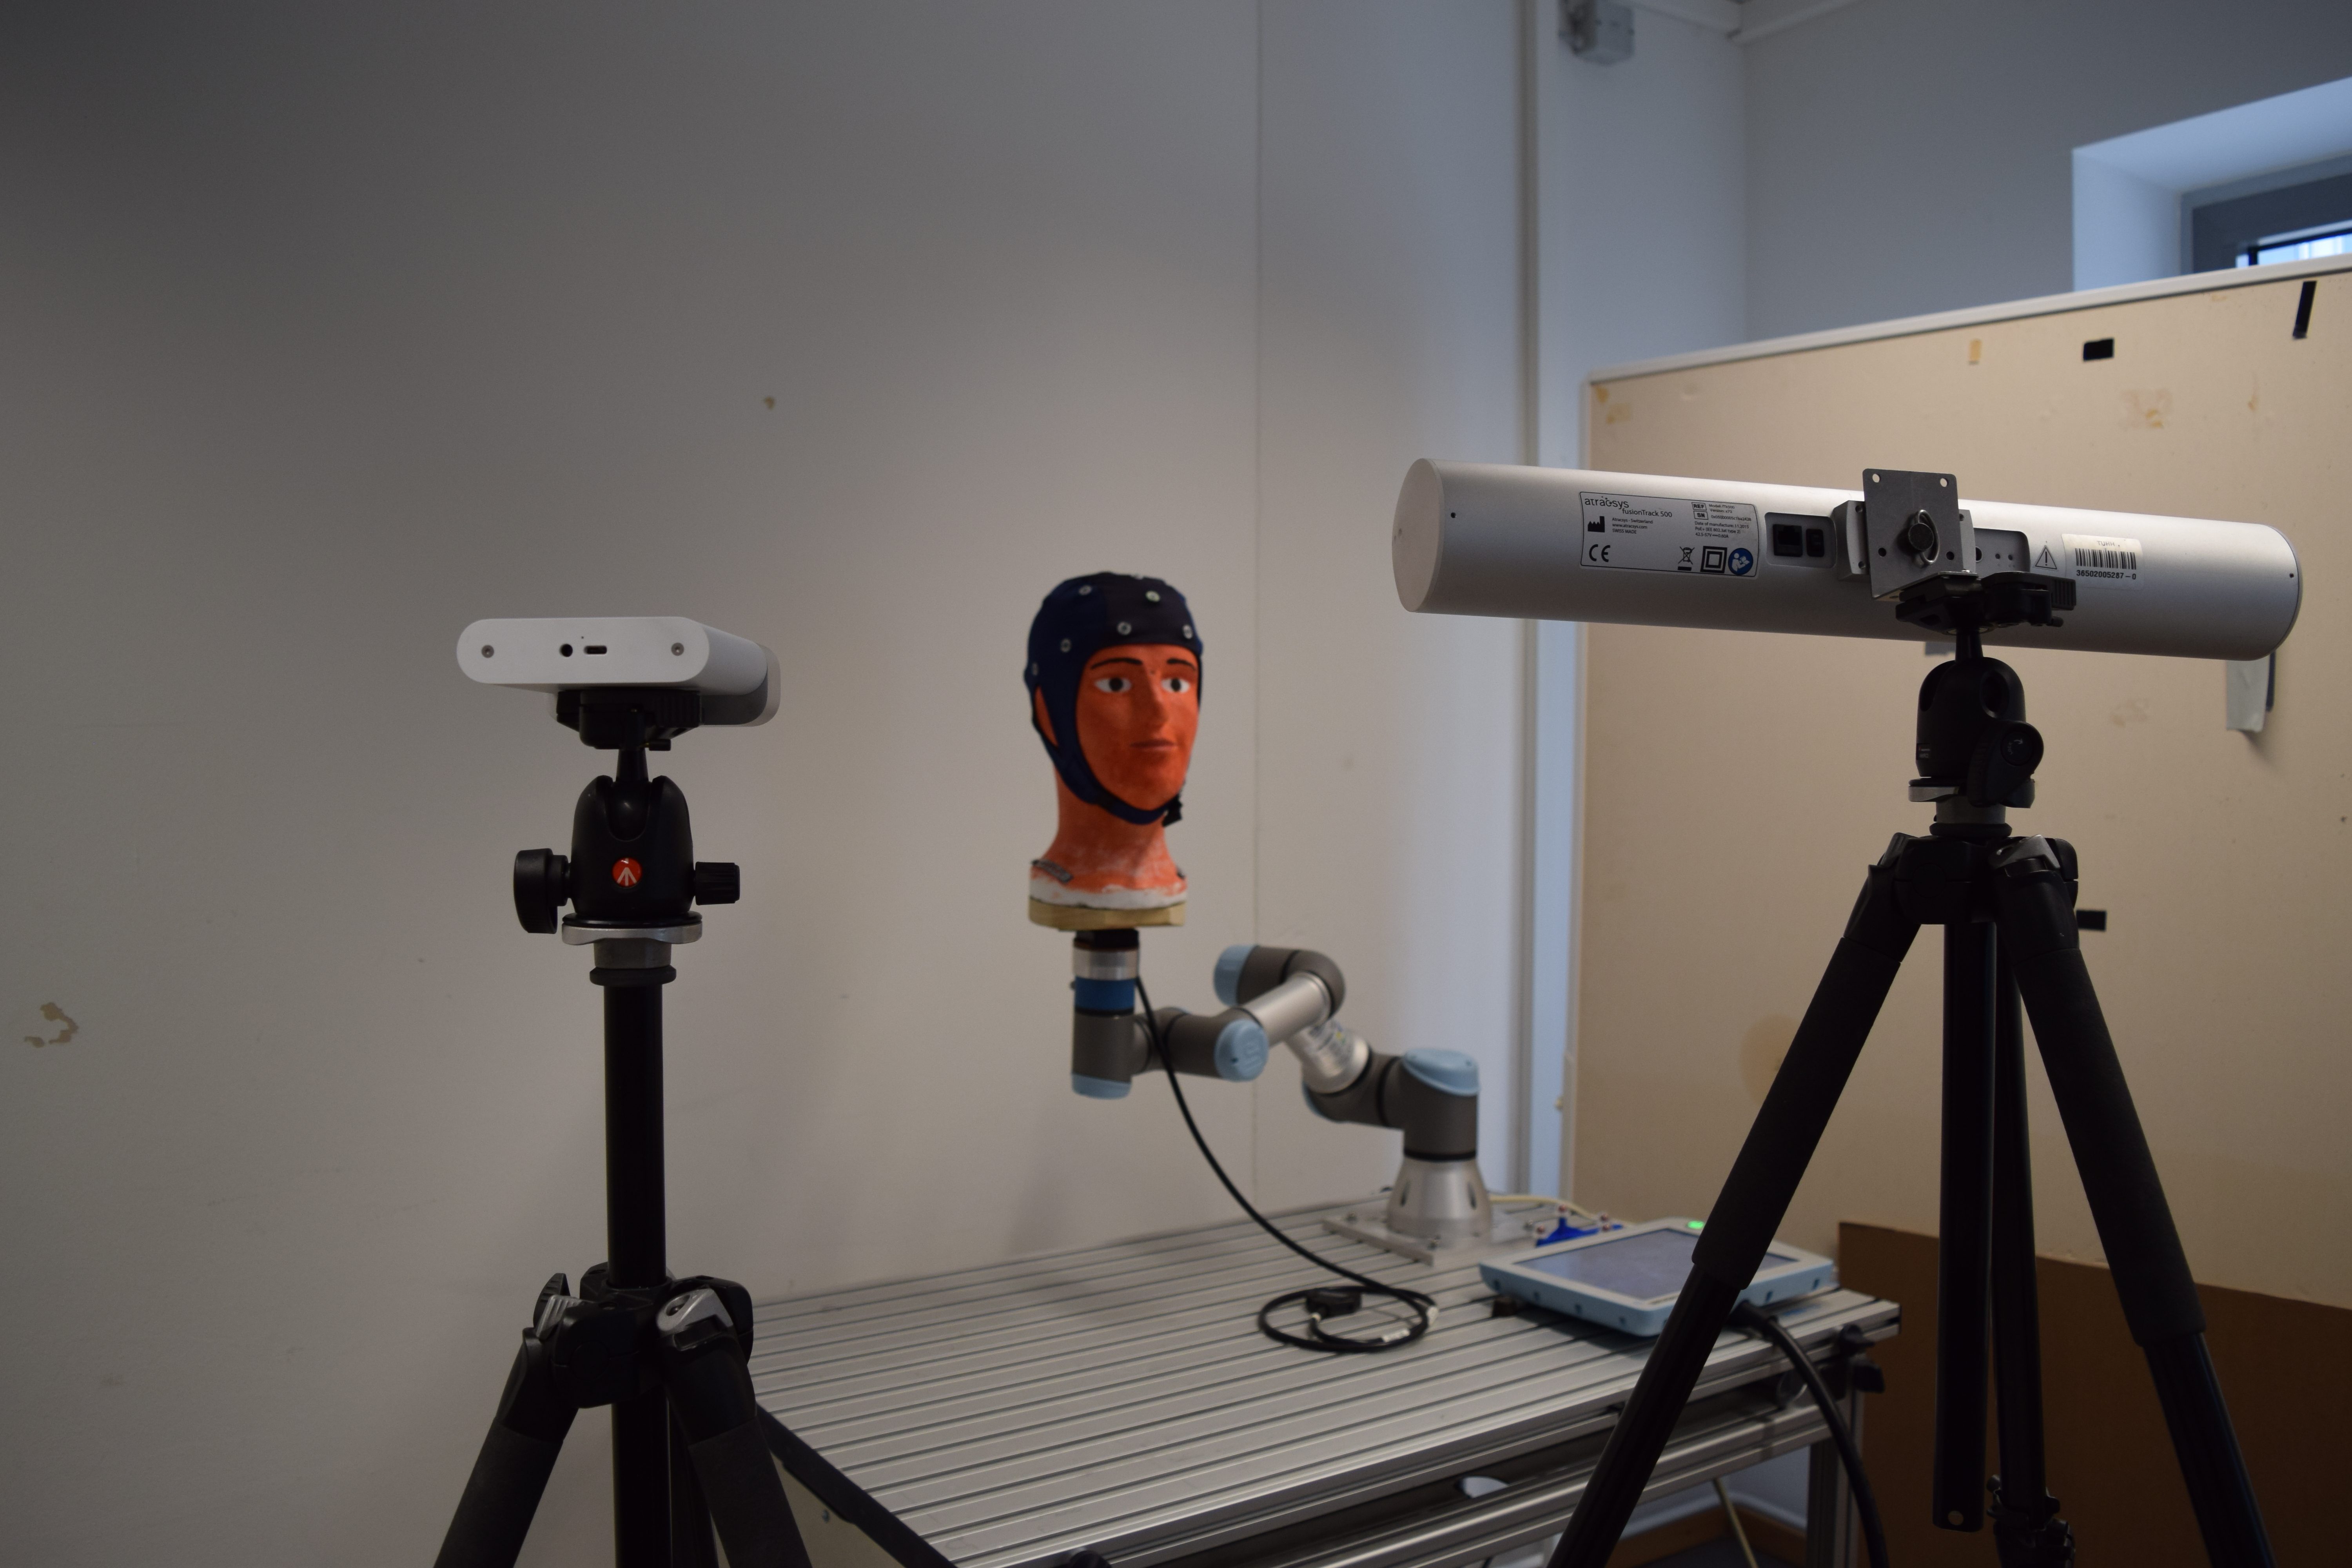
\includegraphics[width=\textwidth]{experimental_setup_1.jpg}	
		\end{subfigure}
		\begin{subfigure}{0.4\textwidth}
			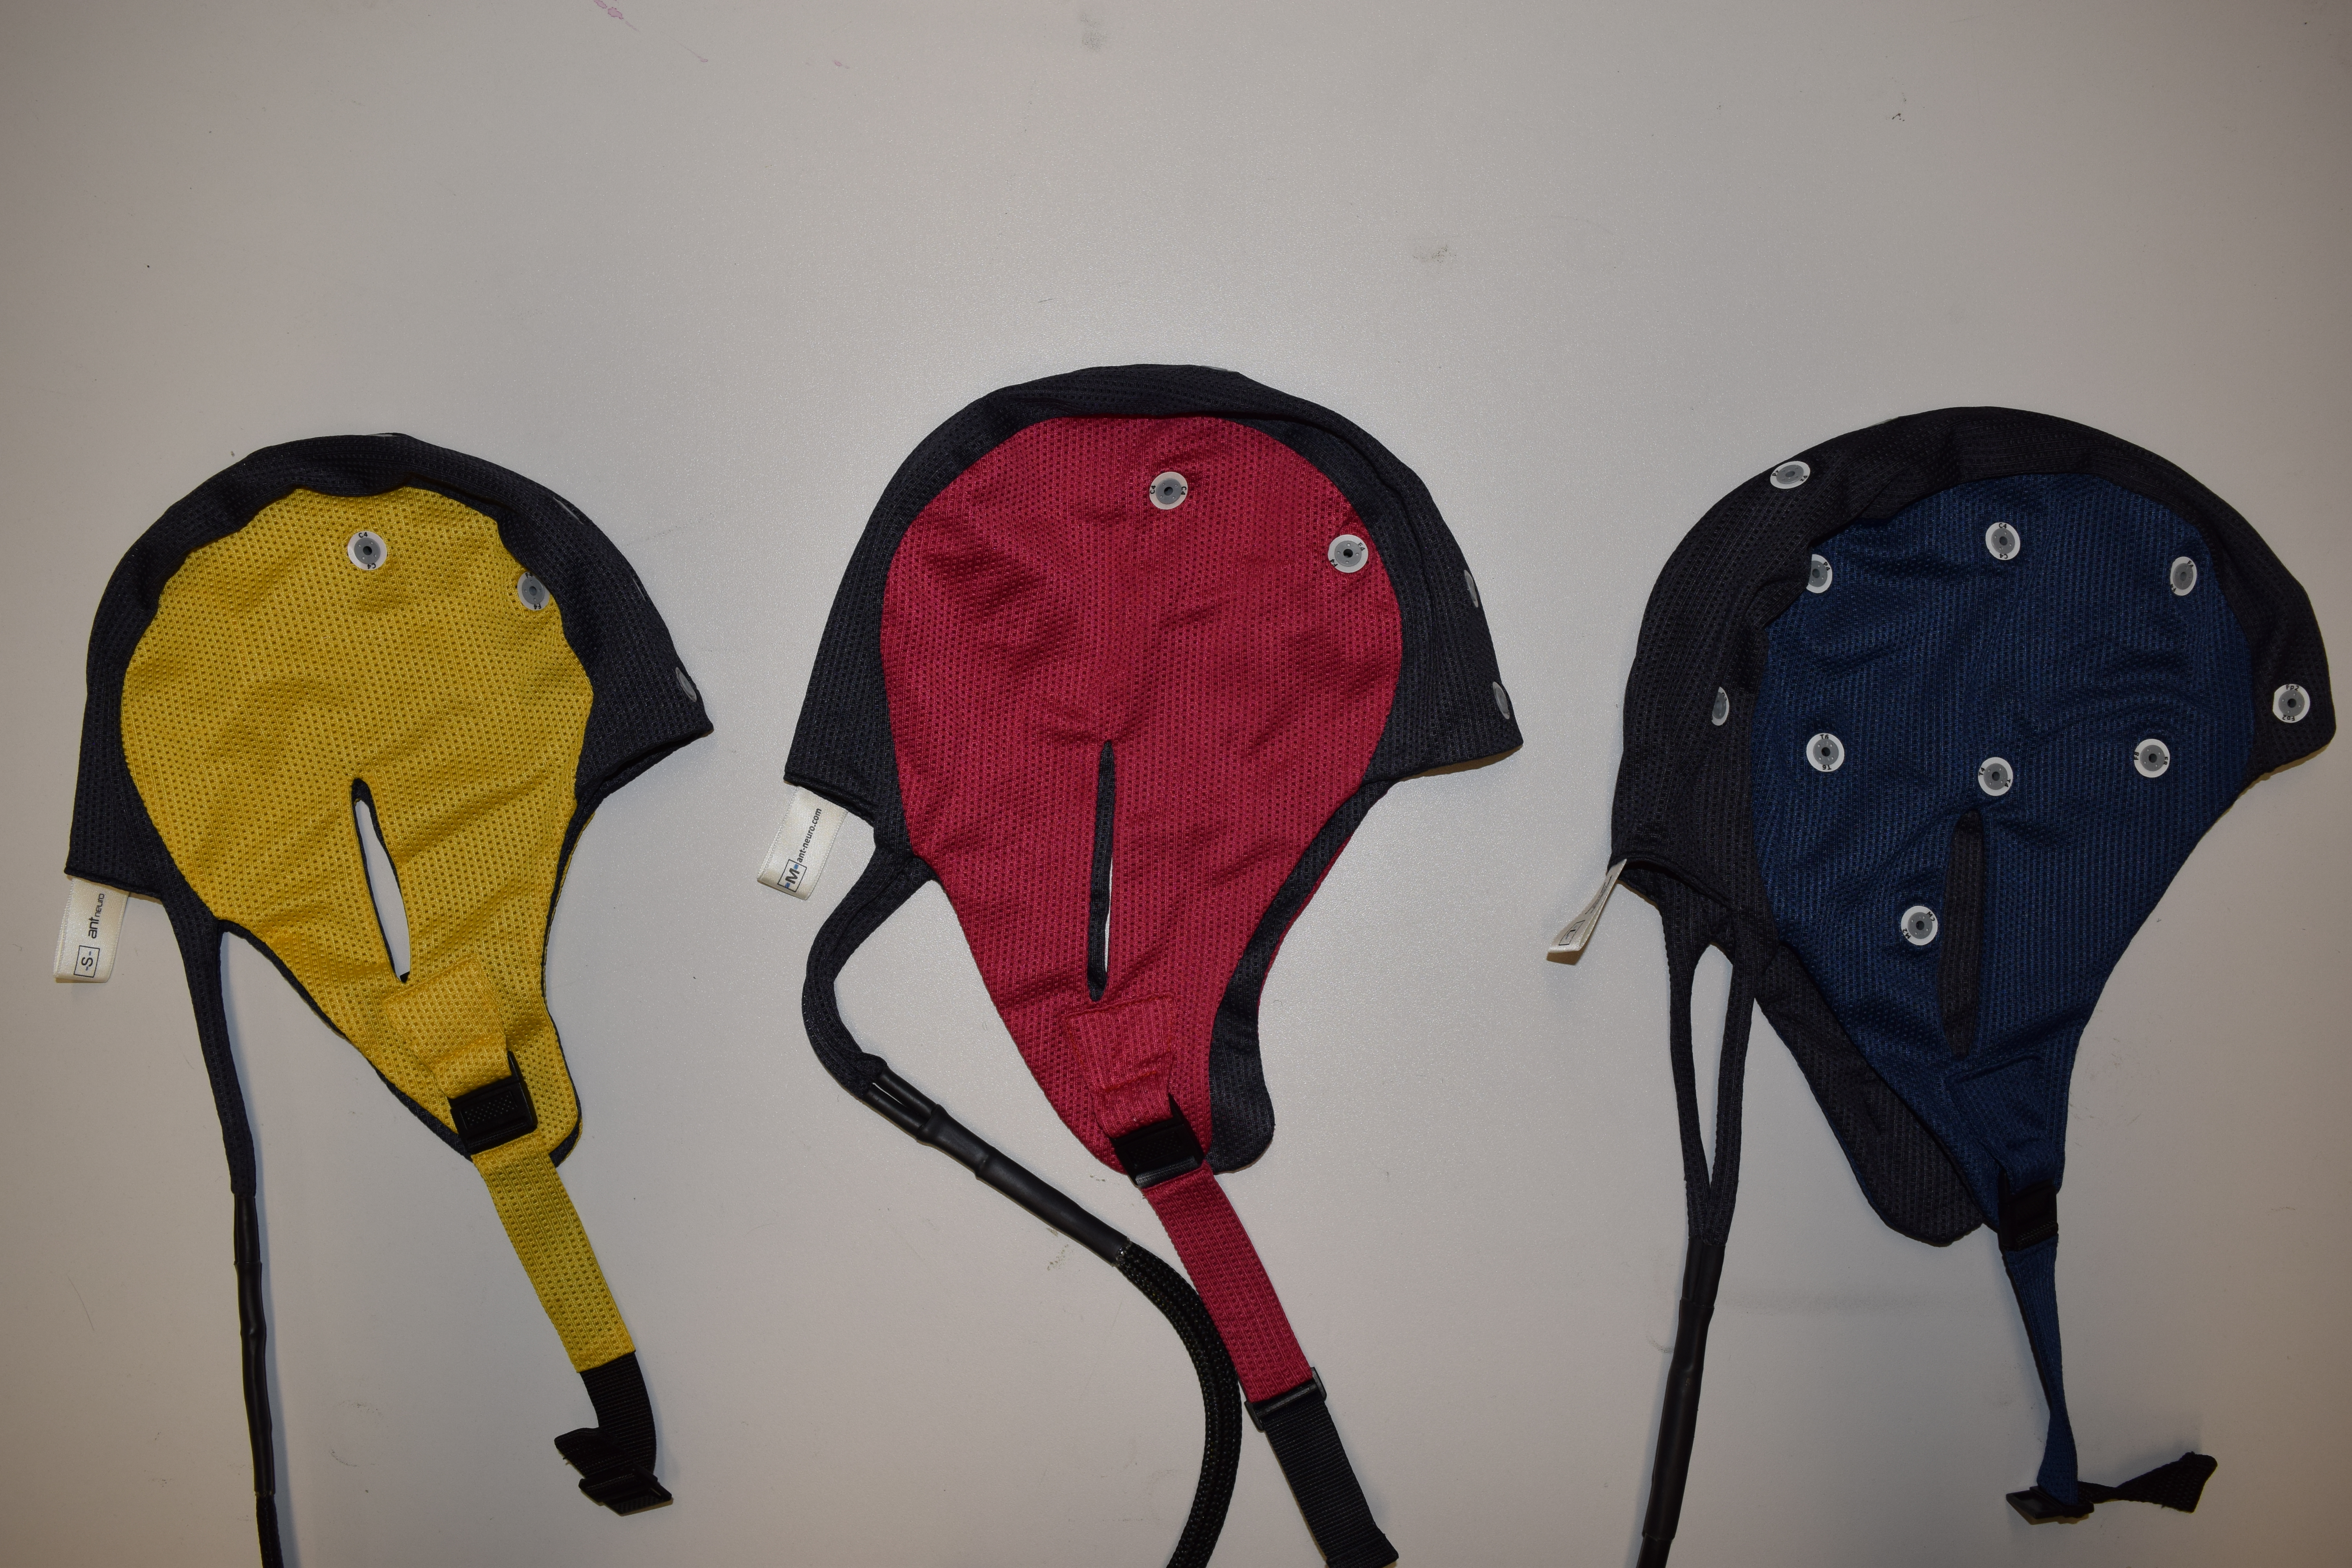
\includegraphics[width=\textwidth]{different_EEG_caps.jpg}	
		\end{subfigure}
		\hfill
		\begin{subfigure}{0.4\textwidth}
			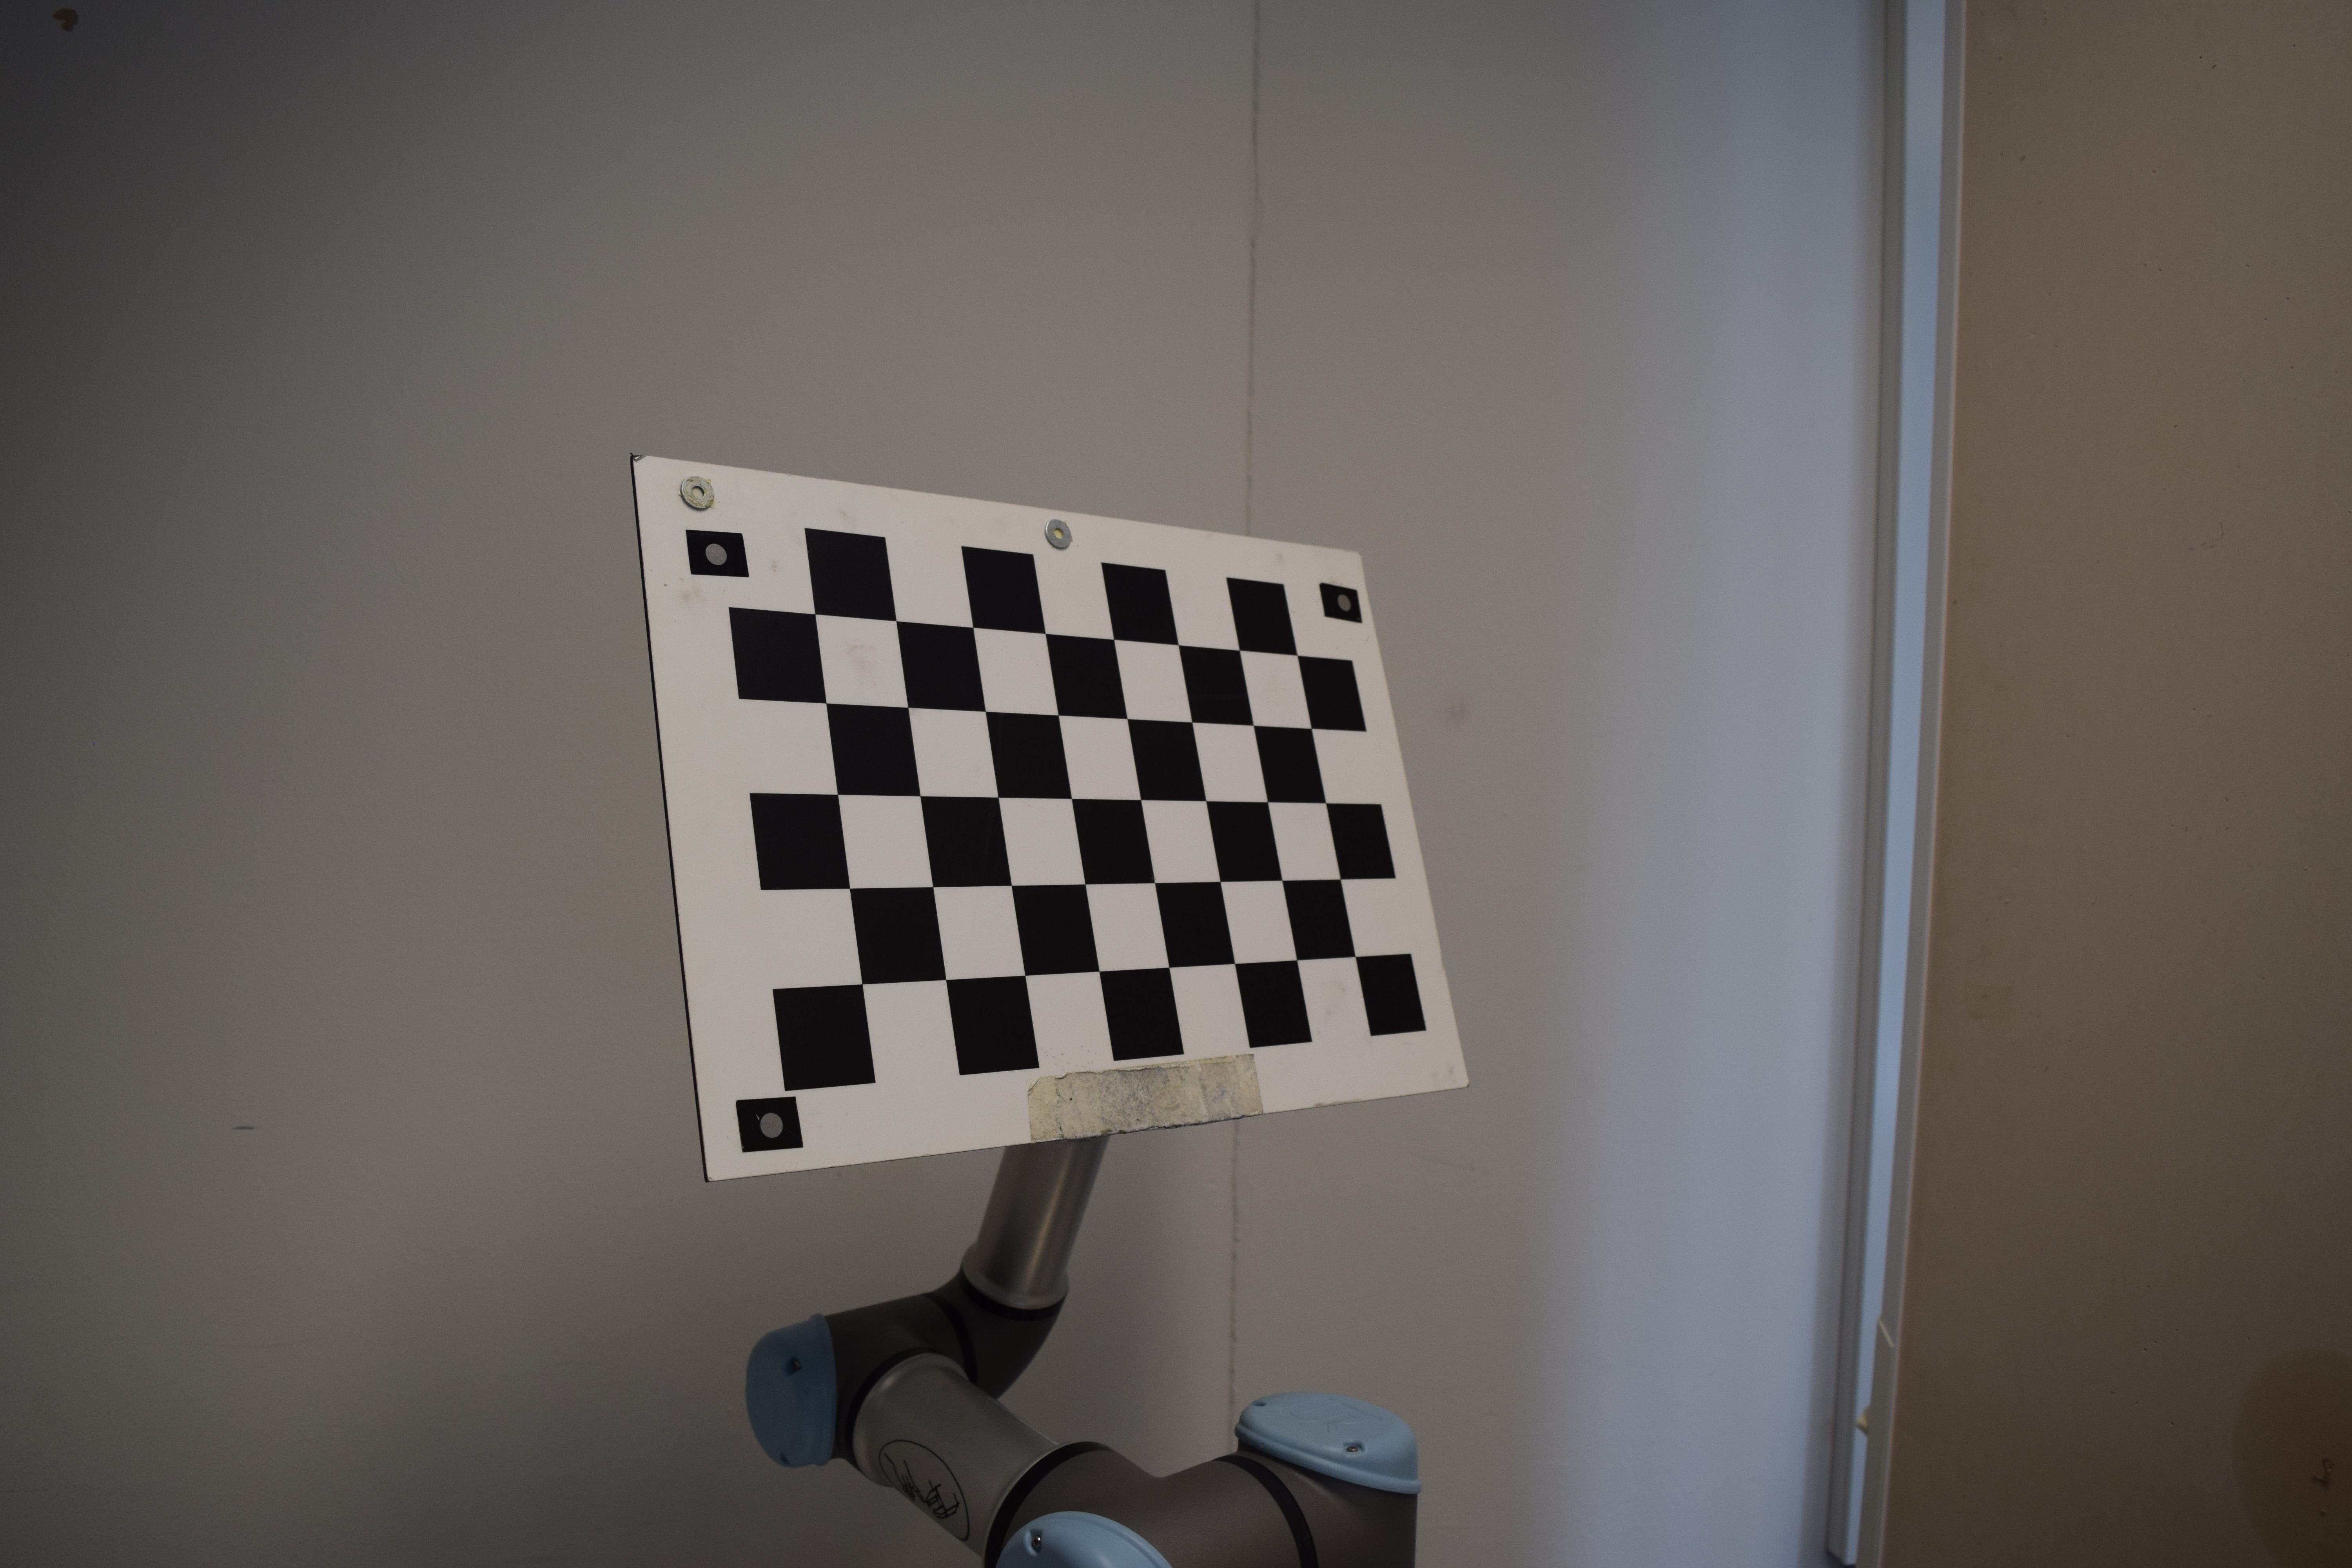
\includegraphics[width=\textwidth]{chessboard.jpg}	
		\end{subfigure}
		\begin{subfigure}{0.4\textwidth}
			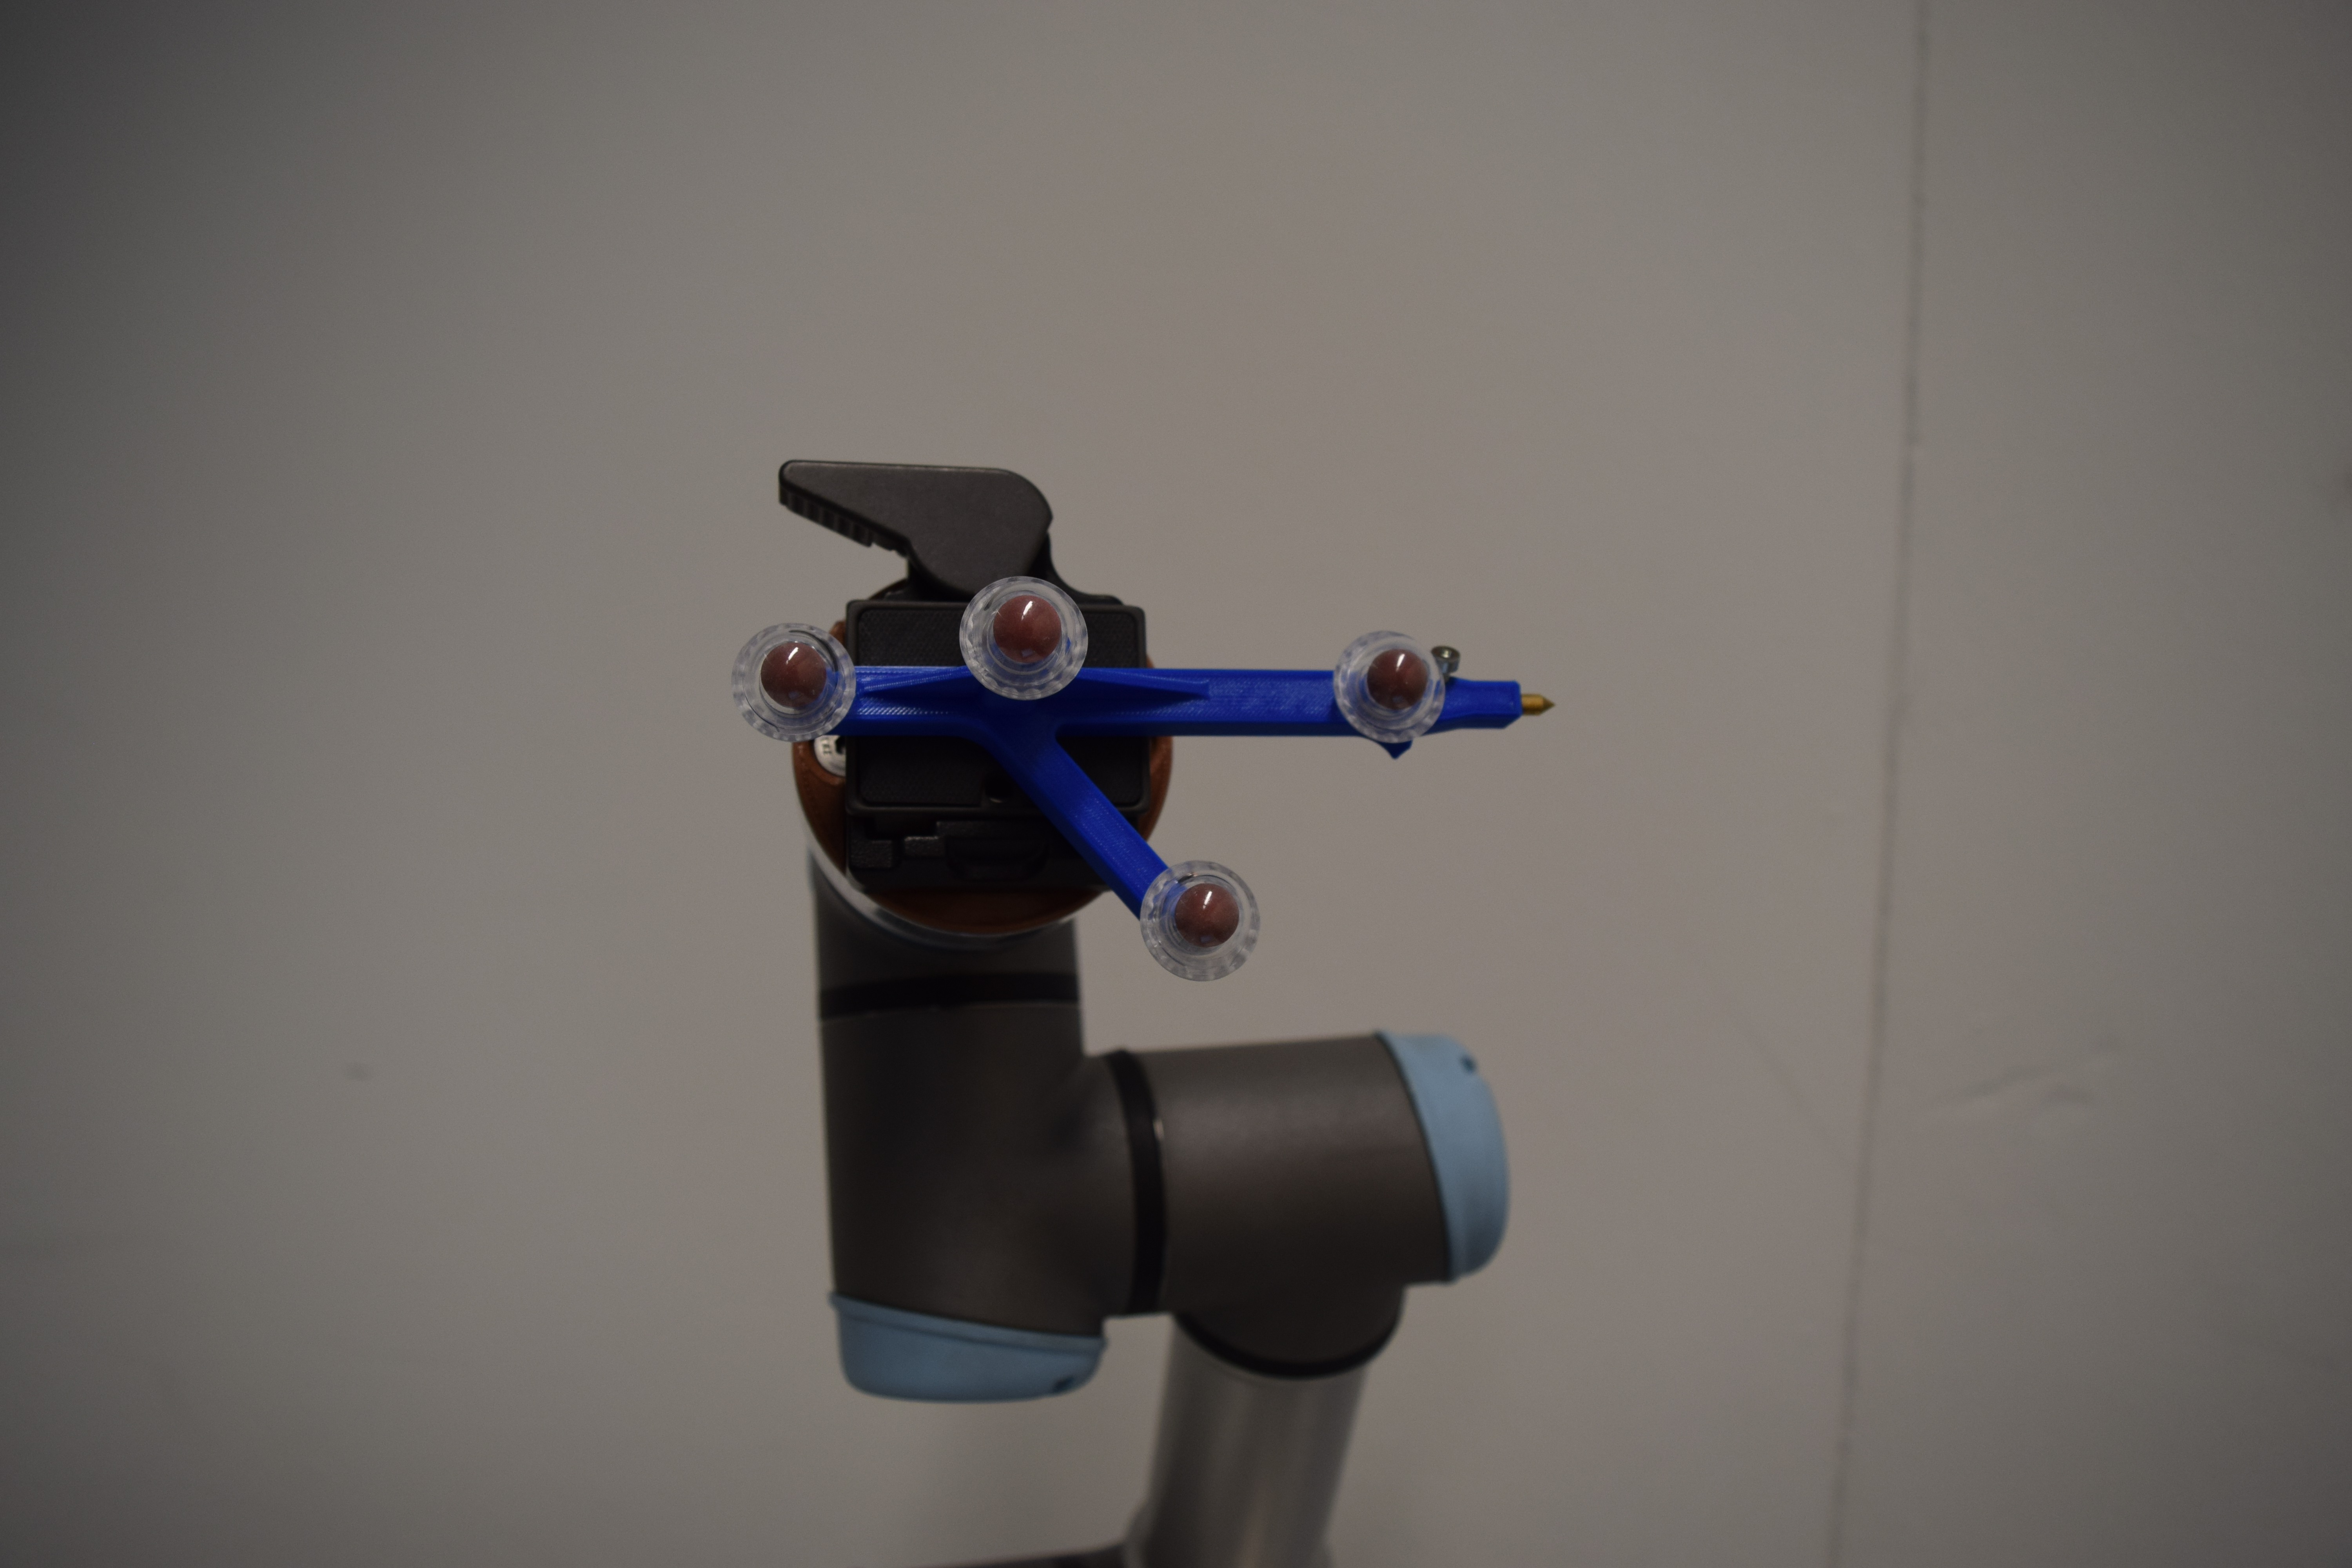
\includegraphics[width=\textwidth]{active_marker.jpg}	
		\end{subfigure}
		
		\caption{Setup consists of Microsoft kinect, Atracsys fusionTrac 500, UR3 robot, EEG caps by eemagine Medical Imaging Solutions GmbH, Berlin, and Markers.} 
		\label{fig:Eexperimental_setup}
	\end{figure}
	
\end{frame}



 

\section{Camera calibration and pose estimation}
Camera calibration is carried out using open-source computer vision library OpenCV \cite{OpenCV}. Camera calibration is based on 2D/2D point correspondences with the chessboard as a 2D planar object. The homography is calculated using square corners of a chessboard (world points) and its image points. OpenCV needs an arrays of world points and image points and the grid size of the chessboard (in our case its 5 rows, 8 columns). Therefore, 10 RGB images of the chessboard at different position and orientation was recorded and an array of world points (x,y) location of chessboard corners [(0,0), (40,0), (80,0)...] was fed to the algorithm. OpenCV automatically detects these chessboard corners from the images as shown in \cref{fig:chessboard_corners} and refines them accordingly.

\begin{figure}[hbt!]
	\centering
	\includegraphics[scale=0.6]{chessboard_corners.png}
	\caption{Chessboard corners(image points) detection in OpenCV}
	\label{fig:chessboard_corners}
\end{figure}

\begingroup\makeatletter\def\@currenvir{verbatim}
\verbatim
cv2.calibrateCamera(object_points, image_points, ...)
output: rms, camera_matrix, dist_coeffs, rot_vecs, trans_vecs
\end{verbatim}

The OpenCV function cv2.calibrateCamera takes in these world points (object points), image points and some more arguements then outputs geometric error of reprojection (rms), intrinsic parameters (camera\_matrix) distortion coefficients (dist\_coeffs) and extrinsic parameters $(rot\_vecs, trans\_vecs)$.

Having completed the camera calibration we can now make use of the intrinsic parameters and the distortion coefficients as an input to the pose estimation algorithm provided by OpenCV. 

\begingroup\makeatletter\def\@currenvir{verbatim}
\verbatim
cv2.solvePnP(object_points, image_points, intr_mat, dist_coeffs)
output: rot_vecs, trans_vecs 
\end{verbatim}


The OpenCV function cv2.solvePnP takes object points, image points, intrinsic matrix, and distortion coeffcients as the arguments and computes rotation and translation vectors. Rotation vector can be converted to 3$\times$3 rotational matrix using cv2.Rodrigues function provided by openCV. By combining rotation matrix and translation vector we can form 4$\times$4 homogenious matrix for further manipulation.
\section{Pre-Data Acquisition steps}
\begin{frame}
	\frametitle{Hand-eye calibration}
	\begin{itemize}
		\item Chessboard pose estimation with new Kinect is integrated to existing hand-eye calibration framework
		\item Results,
		\begin{table}[hbt!]
			\centering
			\begin{tabular}{|c|c|c|}
				\hline
				Camera & Translation error (m) & Rotational error ($\deg$)\\ 
				\hline
				Kinect & 0.001$\pm$ $\num{1.40e-07}$  & 0.258 $\pm$ $\num{0.000}$\\
				fusionTrac & 0.001 $\pm$ $\num{2.8e-07}$  & 0.205 $\pm$ $\num{0.000}$\\
				\hline
			\end{tabular}
			\caption{Hand-eye calibration results}
			\label{tab:kinect__fusionTrac_handeye_result}
		\end{table}
	\end{itemize}
\begin{block}{Exceeded the benchmark }
	Translational error $<$ 1.1 mm and rotational error  $<$ 0.3 degrees.
\end{block}
		
\end{frame}
\section{Pre-Data Acquisition steps}
\begin{frame}
	\frametitle{Head coordinate system}
	\begin{figure}[hbt!]
		\centering
		\includegraphics[scale=0.27]{BTi_4D.png}
		\caption{The BTi/4D coordinate system convention.} 	
	\end{figure}
\begin{itemize}
	\item The origin is between LPA \& RPA
	\item The $\vect{x}$ axis goes through nasion.
	\item The $\vect{y}$ goes through LPA, orthogonal to $\vect{x}$
	\item The $\vect{z}$ axis is orthogonal to both $\vect{x}$ \& $\vect{y}$
\end{itemize}
\end{frame}

\section{Pre-Data Acquisition steps}
\begin{frame}
	\frametitle{Head coordinate system}
	\begin{figure}[hbt!]
	\centering
		\begin{subfigure}{0.25\textwidth}
			\includegraphics[width=\textwidth]{csys_1.png}	
		\end{subfigure}
		\begin{subfigure}{0.25\textwidth}
			\includegraphics[width=\textwidth]{csys_2.png}	
		\end{subfigure}
		\\
		\begin{subfigure}{0.25\textwidth}
			\includegraphics[width=\textwidth]{csys_3.png}	
		\end{subfigure}
		\begin{subfigure}{0.25\textwidth}
			\includegraphics[width=\textwidth]{csys_4.png}	
		\end{subfigure}
	\caption{Vector algebra in head coordinate system creation.} 
	\label{fig:BTi_4D_3}
	\end{figure} 
\end{frame}



\section{Pre-Data Acquisition steps}
\begin{frame}
	\frametitle{Head coordinate system}
	\begin{figure}[hbt!]
		\centering
		\includegraphics[scale=0.30]{head_coordinate.png}
		\caption{Head coordinate system using RPA, nose and LPA} 
		\label{fig:head_coordinate}
	\end{figure}
\end{frame}



\section{Data Acquisition}
\begin{frame}
	\frametitle{Electrode mapping problem}
	We cannot map all the electrodes in the cap without disturbing the head position
	\begin{figure}[hbt!]
		\centering
		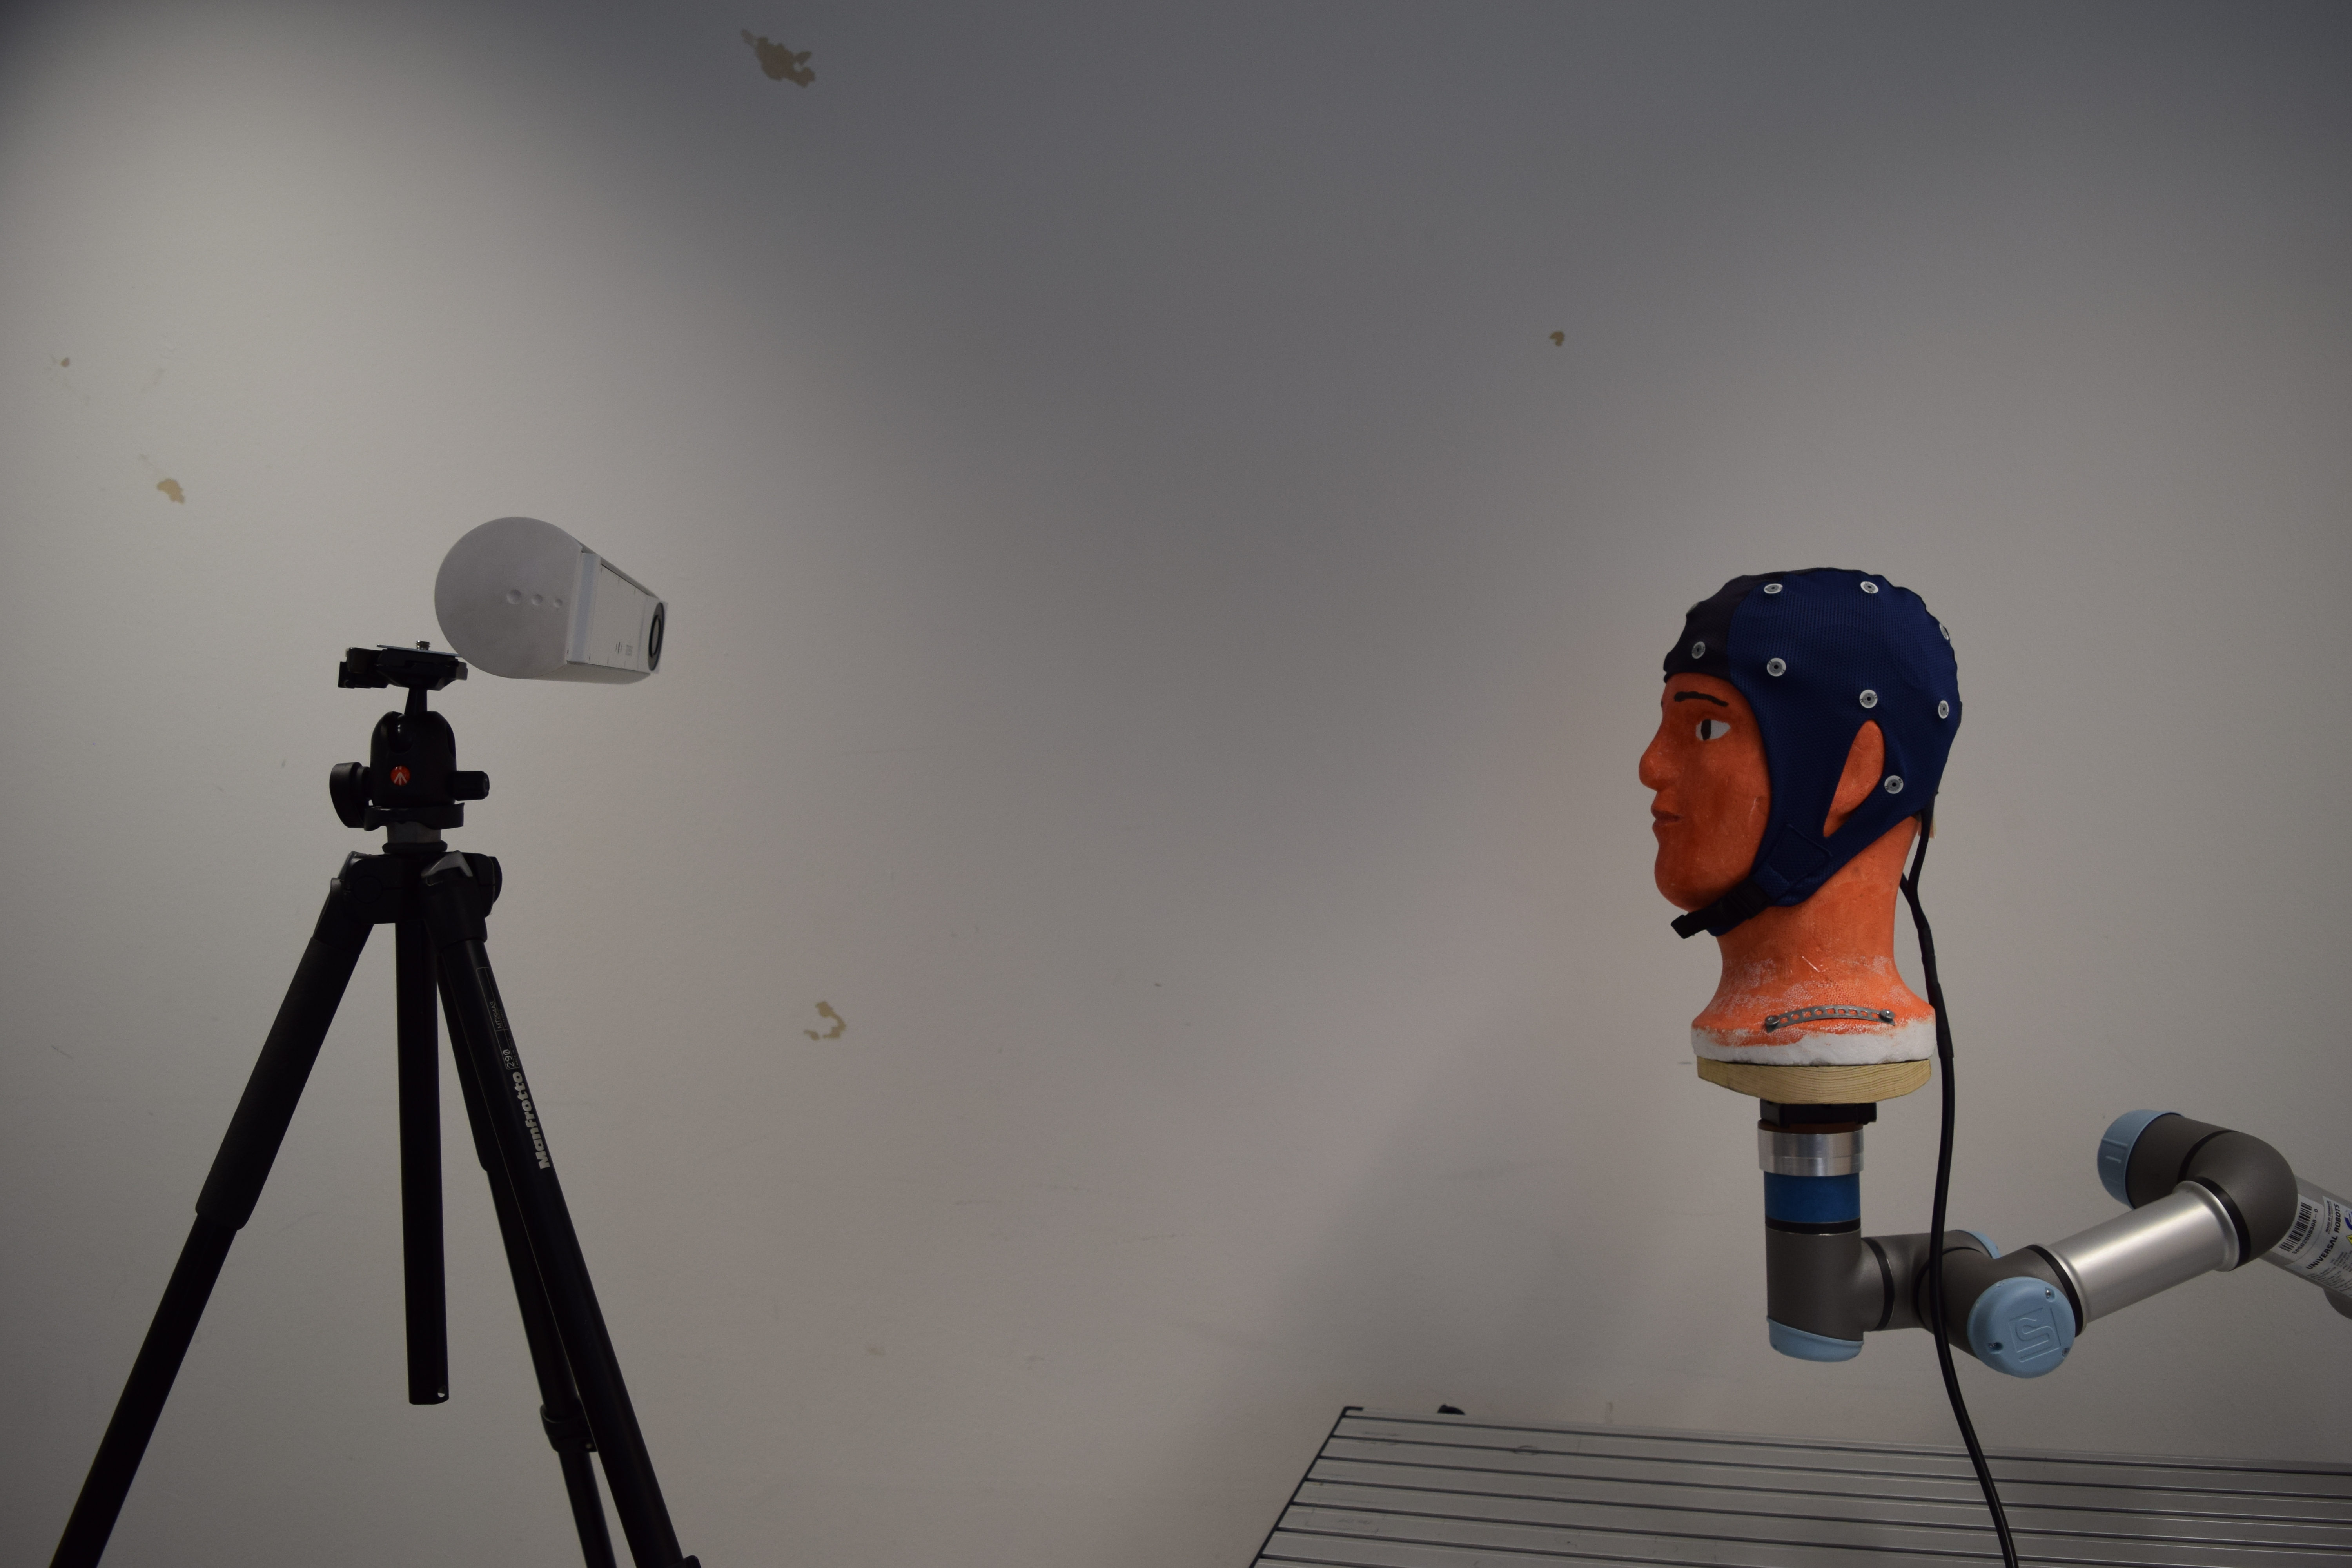
\includegraphics[scale=0.14]{fusionTrac_phantom.jpg}
		\caption{Difficult to capture electrodes at the back of the phantom head.} 
		\label{fig:fusionTrac_phantom}
	\end{figure}
\begin{block}{Decouple}
	decoupling the head coordinate system generation and electrode mapping 
\end{block}
\end{frame}



\section{Data Acquisition}
\begin{frame}
	\frametitle{Electrode mapping solution}
	\begin{itemize}
		\item First tranfer the head coordiante system to the end effector frame
			\begin{equation*}
			\tfMat{EE}{T}{H_{CS}} = \invMat{(\tfMat{Base}{T}{EE})} \tfMat{Base}{T}{fCam} \tfMat{fCam}{T}{H_{CS}}
			\end{equation*}
		\item Record all the electrodes in the end effector frame
			\begin{equation*}
			\tfMat{EE}{T}{electrodes} = \invMat{(\tfMat{Base}{T}{EE})} \tfMat{Base}{T}{fCam} \tfMat{fCam}{T}{electrodes}
			\end{equation*} 
		  \item hhh
		  \begin{equation*}
		  \tfMat{kCam}{T}{electrodes}^j =
		   \invMat{(\tfMat{Base}{T}{kCam})} \tfMat{Base}{T}{EE}^j
		   \tfMat{EE}{T}{electrodes}
			\end{equation*} 
			\item where, j $\in$ N [1,2,.......N]
	\end{itemize}
\begin{block}{solution}
	decoupling allowed head movement during electcode mapping
\end{block}
		
\end{frame}



\section{Accuracy of measurement}
\begin{frame}
	\frametitle{Head movement during electrode mapping}
	\begin{figure}[hbt!]
		\centering
		\begin{subfigure}{0.49\textwidth}
			\includegraphics[width=\textwidth]{phantom_single_axis.png}	
		\end{subfigure}
		\hfill
		\begin{subfigure}{0.49\textwidth}
			\includegraphics[width=\textwidth]{phantom_multiple_axis.png}	
		\end{subfigure}
		\caption{Phantom head rotation along single and multiple axes.} 
		\label{fig:phantom_multiple_axis}
	\end{figure} 
	\begin{itemize}
		\item Transfer all the electrode position to head coordinate system
		\begin{equation*}
		\tfMat{H_{CS}}{T}{electrodes} = \invMat{(\tfMat{EE}{T}{H_{CS}})} \tfMat{EE}{T}{electrodes}
		\end{equation*}
	\end{itemize}

\begin{block}{Error}
	Head movement while mapping introduced an error!
\end{block}
	
\end{frame}



\section{Accuracy of measurement}
\begin{frame}
	\frametitle{Effect of single axis rotation}
	\begin{figure}[hbt!]
		\centering
		\includegraphics[scale=0.5]{normalised_positional_error_single_axis.png}
		\caption{Measurement of single electrode when phantom head roatated to ten different angles along an axis.} 
		\label{fig:Normalised_positional_error_single_axis}
	\end{figure}
	
\begin{block}{measurement error}
		mean value with tolerance 118.26$\pm$4.5mm (SD)
\end{block}
		
\end{frame}



\section{Accuracy of measurement}
\begin{frame}
	\frametitle{Effect of multiple axis rotation}
	\begin{figure}[hbt!]
		\centering
		\includegraphics[scale=0.5]{normalised_positional_error_multiple_axis.png}
		\caption{Measurement of single electrode when phantom head roatated to ten different angles along multiple axes.}  
		\label{fig:Normalised_positional_error_multiple_axis}
	\end{figure}
	
\begin{block}{measurement error}
	mean value with tolerance  116.5$\pm$ 1.5mm.
\end{block}
		
\end{frame}



\section{Accuracy of measurement}
\begin{frame}
	\frametitle{Effect of marker orientation}
	\begin{figure}[hbt!]
		\centering
		\includegraphics[scale=0.5]{active_marker_positional_error_normalised.png}
		\caption{Measurement of single electrode with ten different marker orientation} 
		\label{fig:active_marker_normalised_positional_error}
	\end{figure}
	
\begin{block}{measurement error}
		mean value with tolerance 137.05 $\pm$ 1 mm.
\end{block}
		
\end{frame}



\section{Accuracy of measurement}
\begin{frame}
	\frametitle{Data acquisition}
	\begin{figure}[hbt!]
		\centering
		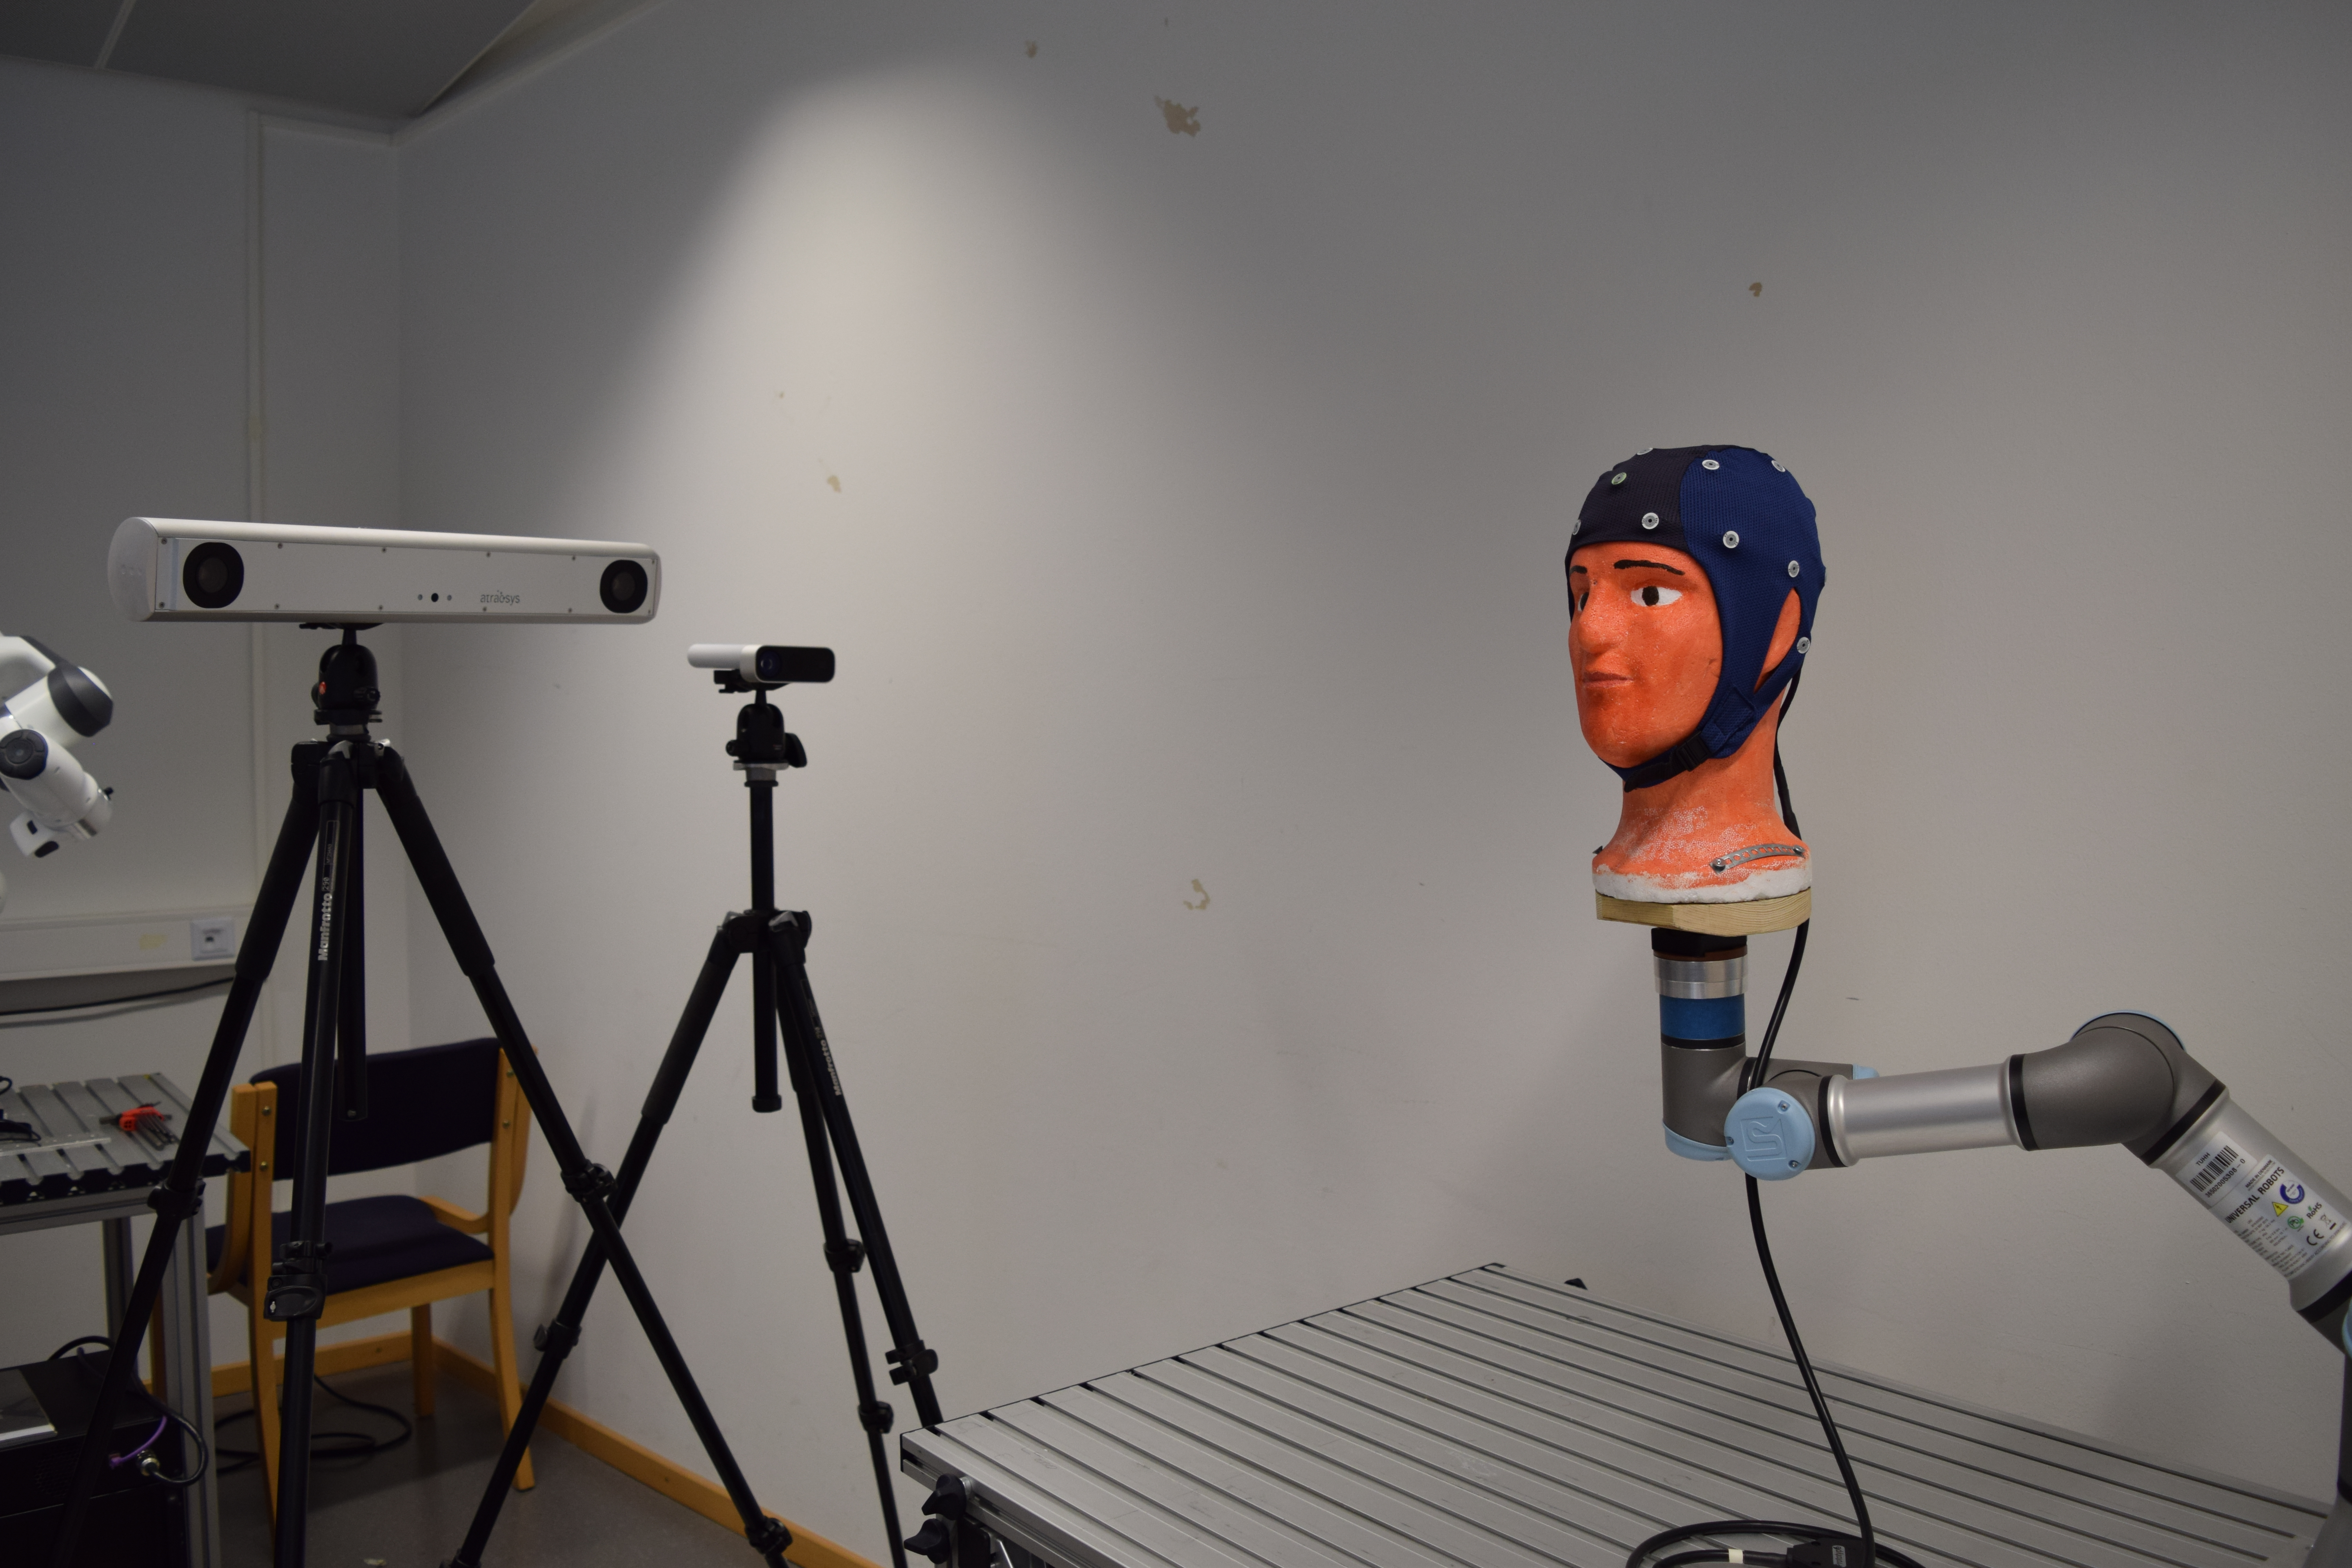
\includegraphics[scale=0.25]{robot_movement.png}
		\caption{360 degrees movement of the phantom head.} 
		\label{fig:robot_movement}
	\end{figure}
	ROS bag record 30-45 seconds video at 30fps.
	\begin{enumerate}
		\item $/k4a/depth\_to\_rgb/camera\_info.$
		\item $/k4a/depth\_to\_rgb/image\_rect.$
		\item $/k4a/rgb/camera\_info.$
		\item $/k4a/rgb/image\_rect\_color.$
		\item $/k4a/points2.$
		\item $joints\_states.$
	\end{enumerate}
		
\end{frame}



\section{visualization}
\begin{frame}
	\frametitle{Electrode position variation}
	\begin{figure}[hbt!]
		\centering
		\includegraphics[width=\linewidth]{blue_cap_all.png}
		\caption{3D view of electrodes at 5 different EEG cap wearing instances} 
		\label{fig:blue_cap_all}
	\end{figure}		
\end{frame}



\section{visualization}
\begin{frame}
	\frametitle{Electrode position variation}
	\begin{figure}[ht!]
		\centering
		\includegraphics[scale=0.6]{electrode_position_range.png}
		\caption{Range of electrode position variation at 5 different EEG cap wearing instances} 
		\label{fig:electrode_position_range}
	\end{figure}
		
\begin{block}{Range of variation}
	mean value with tolerance  7.8 $\pm$ 5.8 mm.
\end{block}

\end{frame}


 
\section{consulsion}
\begin{frame}
	\frametitle{Conclusion}
	\begin{itemize}
		\item New Kinect is integrated successfully
		\item High degree of accuracy is achieved in hand-eye calibration.
		\item Electrode location can be recorded with accuracy of $<$ $\pm$ 5mm
		\item A large amount of ground turth data generated for 3 EEG caps
		\item These data can used for 
		\begin{itemize}
			\item Training and evaluation of CNNs
			\item Evaluation of camera based electrode detection algorithm in general  
		\end{itemize}
		\item Range of electrode position variation for 5 wearing instaces has been exlpored
	\end{itemize}

\end{frame}
\section{consulsion}
\begin{frame}
	\frametitle{Future scope}
	\begin{itemize}
		\item Redesigning the reflective marker that can reach all the electrodes without having to move the phantom
		head.
			\begin{itemize}
				\item Head movement while mapping introduced measurement error of $<$ $\pm$ 5mm.
				\item Current algorithms works any reflective marker.
			\end{itemize}
		\item Filtering system
			\begin{itemize}
				\item Not all the electrodes can be seen in a single image.
				\item The position of all the electrode
				is recorded in the Kinect frame even the ones that are not visible.
			\end{itemize}
	\end{itemize}
\end{frame}
\section{consulsion}
\begin{frame}
	\frametitle{The End}
		  Thanks for your attension!
\end{frame}
\section{Pre-Data Acquisition steps}
\begin{frame}
	\frametitle{Camera calibration}
	\begin{table}[hbt]
		\centering
		\begin{tabular}{|c|c|}
			\hline
			$\tfMat{Base}{T}{EE}$ & M \\
			$\tfMat{EE}{T}{CB}$ & X \\
			$\tfMat{Base}{T}{Cam}$ & Y \\
			$\tfMat{Cam}{T}{CB}$ & N \\
			\hline
		\end{tabular}
	\end{table}
	\begin{equation}
	\matr{M}_i\matr{X} - \matr{Y}\matr{N}_i = 0 
	\label{eq:hand-eye}
	\end{equation}
	\begin{equation}
	\centering
	\begin{split}
	\matr{A} \vect{w} = \vect{b}\\
	\end{split}
	\label{eq:hand-eye_least_square}
	\end{equation}
	\begin{equation}
	\sum_{i=1}^n \|\matr{M}_i\matr{X} - \matr{Y}\matr{N}_i\|_{F}\
	\end{equation}

\end{frame}







\begin{frame}
	\frametitle{Agenda}
	\printbibliography
\end{frame}



\end{document}